\section{Test Environment}

In this question we introduce the test environment which we will be using throughout the rest of the assignment. In particular, we will use this environment to test our code locally before running our code on an Azure instance with a GPU. \\

To start, we will reason about optimality in the provided test environment by hand. Later in the assignment, to sanity-check your code, you will verify that your implementation is able to achieve the optimal return for the test environment. In general, you should be able to run your models in the test enviroment on your machine's CPU in a reasonable amount of time. Below you may find a full specification of the test environment,


\begin{center}
	\begin{tabular}{| p{0.1\linewidth} | p{0.75\linewidth} |}
	\hline
	\textbf{Feature} & \textbf{Specification} \\ \hline
	States & There are four states in total: \{0,1,2,3\} \\[2ex] \hline
	Actions & \makecell[l]{There are five actions in total: \{0,1,2,3,4\}. \\ Actions $ 0 \leq i \leq 3 $ makes the agent go to state $ i $. \\ Action $ 4 $ makes the agent stay in the same state.} \\[2ex] \hline
	Rewards & \makecell[l]{Going to state $ i $ from states 0, 1 and 3 gives a reward $R(i) $, where \\ $R(0) = 0.2$ \\ $R(1) = -0.1$ \\ $R(2) = 0.0$ \\ $R(3) = -0.3$ \\ If we start in state $ 2 $, then the rewards defined above are multiplied by $ - 10 $.}   \\[2ex] \hline
	Episodes & One episode lasts 5 time steps (for a total of 5 actions) and always starts in state $ 0 $ (no rewards at the initial state). \\[2ex] \hline
	\end{tabular}
	\captionof{table}{Specification of features for the test environment}
	\label{table:test_spec_1}
\end{center}

\begin{center}
	\begin{tabular}{ | p{0.2\linewidth} | p{0.2\linewidth} | p{0.2\linewidth} | p{0.2\linewidth} |}
		\hline
		\textbf{State ($s$)} & \textbf{Action ($a$)} & \textbf{Next State ($s'$)} & \textbf{Reward ($R$)} \\ \hline
		0 & 0 & 0 & 0.2    \\ \hline
		0 & 1 & 1 & -0.1   \\ \hline
		0 & 2 & 2 & 0.0 \\ \hline
		0 & 3 & 3 & -0.3 \\ \hline
		0 & 4 & 0 & 0.2 \\ \hline
		1 & 0 & 0 & 0.2    \\ \hline
		1 & 1 & 1 & -0.1   \\ \hline
		1 & 2 & 2 & 0.0 \\ \hline
		1 & 3 & 3 & -0.3 \\ \hline
		1 & 4 & 1 & -0.1 \\ \hline
		2 & 0 & 0 & -2.0    \\ \hline
		2 & 1 & 1 & 1.0   \\ \hline
		2 & 2 & 2 & 0.0 \\ \hline
		2 & 3 & 3 & 3.0 \\ \hline
		2 & 4 & 2 & 0.0 \\ \hline
		3 & 0 & 0 & 0.2    \\ \hline
		3 & 1 & 1 & -0.1   \\ \hline
		3 & 2 & 2 & 0.0 \\ \hline
		3 & 3 & 3 & -0.3 \\ \hline
		3 & 4 & 3 & -0.3 \\ \hline    
	\end{tabular}
	\captionof{table}{Transition table for the test environment}
	\label{table:test_spec_2}
\end{center}

\clearpage
An example of a trajectory (or episode) in the test environment is shown in Figure \ref{fig:test_env}, and the trajectory can be represented in terms of $s_t, a_t, R_t$ as: 
\begin{align*}
\begin{split}
& s_0 = 0, a_0=1, R_0 = -0.1, s_1=1, a_1=2, R_1 = 0.0, s_2=2, a_2=4, R_2 = 0.0, s_3=2, a_3=3, R_3  = 3.0, \\
& s_4=3, a_4=0, R_4 = 0.2, s_5=0
\end{split}
\end{align*}

\begin{figure}[H]
  \centering
  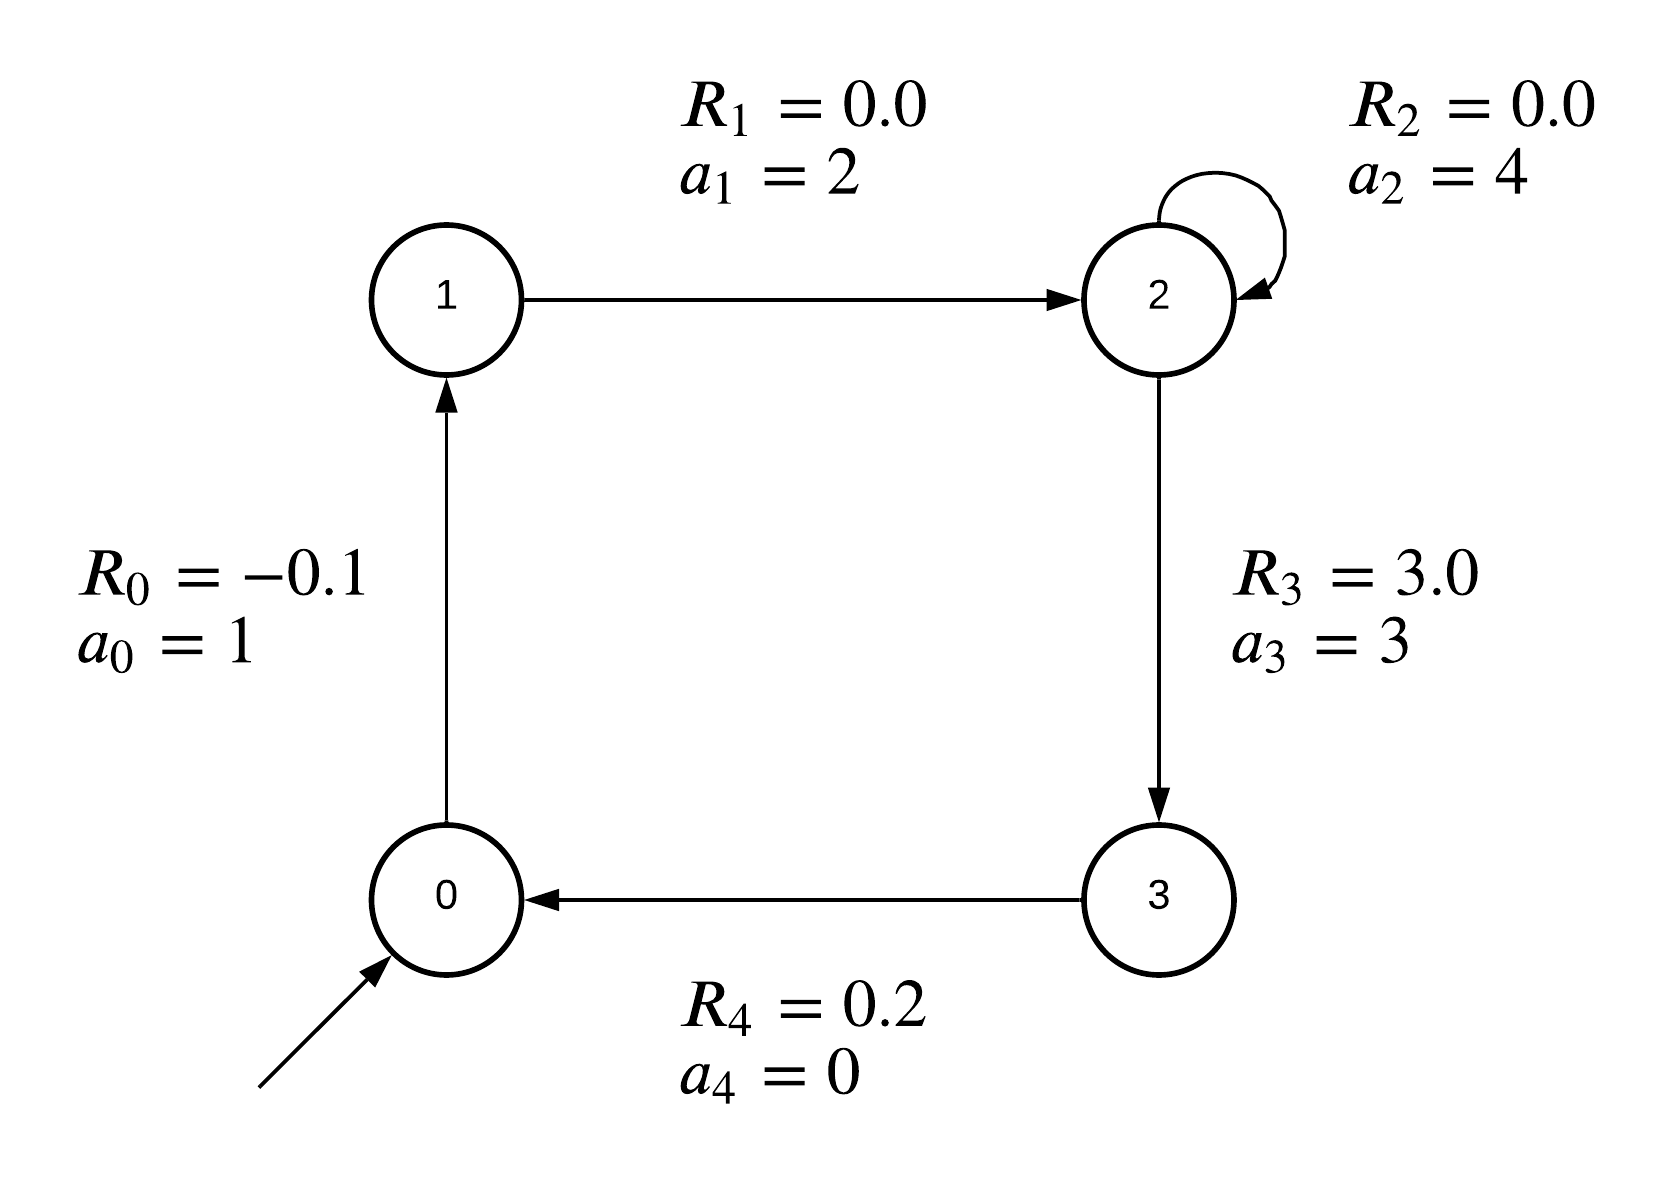
\includegraphics[width=.45\linewidth]{images/test_env.png}
  \caption{Example of a trajectory in the Test Environment}
  \label{fig:test_env}
\end{figure}

\begin{enumerate}[(a)]

	\input{02-test-environment/01-max-rewards}

\end{enumerate}